\documentclass[conference]{IEEEtran}
\IEEEoverridecommandlockouts

\usepackage{cite}
\usepackage{amsmath,amssymb,amsfonts}
\usepackage{algorithmic}
\usepackage{graphicx}
\usepackage{textcomp}
\usepackage{xcolor}
\usepackage{booktabs}
\usepackage{tikz}
\usetikzlibrary{arrows.meta, positioning, shapes.geometric, shapes.misc, fit, backgrounds, calc}
\usepackage{microtype}
\usepackage[hyphens]{url}
\usepackage{hyperref}
\hypersetup{
    colorlinks=true,
    linkcolor=blue,
    citecolor=blue,
    urlcolor=blue
}

\def\BibTeX{{\rm B\kern-.05em{\sc i\kern-.025em b}\kern-.08em
    T\kern-.1667em\lower.7ex\hbox{E}\kern-.125emX}}

\begin{document}

\title{MultiAgentTopologyEval: A Multi-Agent LLM Architecture Evaluation Framework}

\author{\IEEEauthorblockN{Kshitij Kejriwal}
\IEEEauthorblockA{\textit{Department of Computer Applications} \\
\textit{Veermata Jijabai Technological Institute (VJTI)}\\
Mumbai, India}
}

\maketitle

\begin{abstract}
Large Language Model (LLM) agents are increasingly organized into multi-agent systems to solve complex tasks through role specialization and inter-agent collaboration. However, the choice of communication topology---how information flows between agents---remains poorly understood in terms of its holistic trade-offs across task performance, computational cost, execution latency, and runtime reliability. Most existing agent benchmarks evaluate monolithic task completion or simulate complex game environments, leaving the fine-grained operational trade-offs of canonical interaction graphs largely uncharacterized under controlled conditions. 

In this paper, we introduce \textbf{MultiAgentTopologyEval}, a modular and reproducible empirical evaluation framework designed to systematically isolate and profile the operational behavior of five canonical multi-agent topologies: \textsc{Single}, \textsc{Chain}, \textsc{Star}, \textsc{Tree}, and \textsc{Graph}. Rather than focusing solely on binary success, our framework instruments multi-dimensional telemetry capturing decoupled prompt and completion token usage, real-time financial API cost, step-level latency distributions, deterministic constraint satisfaction rates, and operational failure taxonomies (including API rate-limit stalls, request timeouts, schema parsing exceptions, and non-terminating communication loops). 

We evaluate these architectures across seven diverse reasoning, planning, and synthesis task categories over 175 live cloud executions (spanning Google Gemini, Cohere Command, and Groq Llama-3.3) alongside offline deterministic mock baselines. Our empirical findings demonstrate that while centralized (\textsc{Star}) and hierarchical (\textsc{Tree}) topologies prevent single-point failures, linear pipelines (\textsc{Chain}) suffer from cascading constraint degradation. Furthermore, multi-agent coordination incurs a 6.7$\times$ to 7.5$\times$ latency overhead and up to a 15.3$\times$ token amplification compared to an isolated \textsc{Single} baseline, highlighting the critical necessity of multi-dimensional operational profiling when selecting agent architectures.
\end{abstract}

\begin{IEEEkeywords}
Multi-Agent Systems, Large Language Models, Communication Topologies, Empirical Benchmarking, Operational Profiling, Reliability Engineering.
\end{IEEEkeywords}



\section{Introduction}
\label{sec:introduction}

The emergence of Large Language Models (LLMs) built upon Transformer self-attention mechanisms~\cite{Vaswani2017Attention,Devlin2019BERT,Brown2020Language} has driven a fundamental transition in artificial intelligence: moving from passive text generation toward active, goal-directed autonomous agents~\cite{Wang2024Survey,Xi2025Rise}. Equipping foundation models with deliberative reasoning loops (such as Chain-of-Thought~\cite{Wei2022Chain} and ReAct~\cite{Yao2023ReAct}), external working memory~\cite{Park2023Generative,Sumers2024Cognitive}, and API tool execution~\cite{Schick2023Toolformer,Qin2024ToolLLM,Patil2024Gorilla} enables autonomous agents to iteratively decompose and solve complex problems in dynamic software environments.

Despite these advancements, monolithic single-agent systems encounter severe operational and cognitive bottlenecks when confronted with multi-faceted, high-dimensional objectives. Single agents frequently suffer from prompt context saturation, persona drift across extended multi-turn exchanges, and an inability to execute parallel specialization~\cite{Wu2024AutoGen,Li2023CAMEL}. These limitations have catalyzed the rapid evolution of Multi-Agent Systems (MAS)~\cite{Hong2024MetaGPT,Chen2024AgentVerse,Qian2024Communicative}, wherein multiple specialized LLM agents (e.g., Planner, Researcher, Analyst, Critic, and Finalizer) coordinate within structured communication networks to achieve common goals.

\subsection{The Role of Interaction Topology}
In multi-agent orchestration, the \textit{interaction topology}---the directed communication graph defining message routing channels, task delegation hierarchies, and feedback pathways---serves as the primary structural governor of execution behavior. Literature identifies several canonical collaboration topologies:
\begin{itemize}
    \item \textbf{\textsc{Single}} represents the isolated baseline control where a single model processes instructions in a closed turn.
    \item \textbf{\textsc{Chain}} implements a sequential pipeline ($A_1 \rightarrow A_2 \rightarrow \dots \rightarrow A_n$) following standard operating procedures (SOPs)~\cite{Hong2024MetaGPT}.
    \item \textbf{\textsc{Star}} organizes agents into a hub-and-spoke centralized architecture where a central coordinator delegates sub-tasks to specialized satellite workers~\cite{Wu2024AutoGen}.
    \item \textbf{\textsc{Tree}} decomposes objectives through multi-tier hierarchical delegation from root directors down to intermediate leads and leaf execution agents~\cite{Chen2024AgentVerse,Zhu2025MultiAgentBench}.
    \item \textbf{\textsc{Graph}} provides a general mesh network supporting peer-to-peer communicative consensus, cyclic critiques, and dynamic debate loops~\cite{Du2024Improving,Zhu2025MultiAgentBench}.
\end{itemize}

While interaction topology intuitively influences problem-solving quality, its systemic trade-offs remain poorly quantified. Adding communication edges and verification stages can improve factual rigor, but each additional hop incurs compounding wall-clock latency, token explosion, API financial expenditure, and increased vulnerability to runtime operational faults (such as HTTP 429 rate-limit breaches, JSON schema parsing exceptions, provider timeouts, and infinite agent loops).

\subsection{Limitations of Existing Benchmarks}
Existing agent benchmarks, such as AgentBench~\cite{Liu2024AgentBench}, SWE-bench~\cite{Jimenez2024SWEbench}, WebArena~\cite{Zhou2024WebArena}, and GAIA~\cite{Mialon2024GAIA}, have primarily targeted single-agent problem solving within specific digital environments (e.g., operating system shells or web navigation). Recently, Zhu et al.~\cite{Zhu2025MultiAgentBench} introduced \textit{MultiAgentBench} (powered by the MARBLE engine), representing a foundational advance by evaluating multi-agent collaboration and competition across interactive scenarios (such as Minecraft construction and Werewolf social deduction games).

However, current evaluation methodologies exhibit critical operational limitations:
\begin{enumerate}
    \item \textit{Coupled Architectures:} Multi-agent frameworks frequently evaluate their proprietary systems (e.g., MetaGPT's fixed SOP pipeline~\cite{Hong2024MetaGPT} or ChatDev's waterfall phase chat~\cite{Qian2024Communicative}) without systematically isolating the pure effect of interaction topology from the underlying model prompt template.
    \item \textit{Coarse-Grained Operational Metrics:} Existing benchmark suites predominantly report high-level task success rates or milestone KPIs, while leaving step-level execution latency distributions, decoupled prompt versus completion token consumption, and financial API expenditures under-characterized.
    \item \textit{Absence of Runtime Failure Telemetry:} Benchmarks generally treat failed tasks as binary non-completions, omitting structured diagnostics for production runtime exceptions (such as API rate limits, malformed JSON schemas, network timeouts, and circular messaging).
    \item \textit{Environmental Weight and Non-Determinism:} Relying on complex game simulators introduces significant execution noise, heavy local dependencies, and severe computational barriers that hinder reproducible academic benchmarking.
\end{enumerate}

\subsection{Contributions of This Work}
To address these gaps, we propose \textbf{MultiAgentTopologyEval}, a controlled empirical evaluation and operational profiling framework designed to systematically isolate and compare multi-agent LLM interaction topologies. MultiAgentTopologyEval does not introduce a new foundational language model or claim to invent topology evaluation; rather, it provides an open-source, reproducible evaluation testbed that instruments fine-grained systems-level telemetry.

The principal contributions of this work are as follows:
\begin{itemize}
    \item \textbf{Controlled Multi-Topology Harness:} We design a standardized execution engine that evaluates identical task instances across five canonical topologies (\textsc{Single}, \textsc{Chain}, \textsc{Star}, \textsc{Tree}, and \textsc{Graph}) under unified prompt budgets and identical model backends.
    \item \textbf{Comprehensive Multi-Dimensional Telemetry:} We formulate an evaluation suite spanning objective task success, deterministic Constraint Satisfaction Rates (CSR), decoupled prompt/completion token usage, financial API cost modeling, and automated runtime failure tracking (covering rate limits, timeouts, schema violations, and loop traps).
    \item \textbf{Standardized Benchmark Dataset with Anti-Leakage:} We introduce a suite of 7 multi-step technical benchmark tasks spanning planning, constraint balancing, information synthesis, reasoning, decision making, incident response, and algorithmic coding, with strict evaluator ground-truth isolation.
    \item \textbf{Extensive Empirical Profiling:} We report findings across 175 live cloud executions (spanning Google Gemini 3.1 Flash-Lite, Cohere Command, and Groq Llama-3.3-70B) alongside a zero-cost deterministic offline mock mode, quantifying the precise Pareto frontiers of multi-agent orchestration.
\end{itemize}

The remainder of this paper is organized as follows. Section~\ref{sec:related_work} surveys foundational and contemporary literature. Section~\ref{sec:problem_statement} formalizes the research problem and hypotheses. Section~\ref{sec:framework} details the proposed system architecture. Section~\ref{sec:topologies} formalizes the five canonical topologies. Section~\ref{sec:metrics} defines the mathematical metric formulations. Section~\ref{sec:methodology} and Section~\ref{sec:implementation} describe experimental methodology and software design. Section~\ref{sec:results} presents empirical findings. Section~\ref{sec:discussion} discusses architectural trade-offs, followed by threats to validity (Section~\ref{sec:threats_to_validity}), limitations (Section~\ref{sec:limitations}), and conclusions (Section~\ref{sec:conclusion}).


\section{Related Work}
\label{sec:related_work}

\subsection{Foundations of LLM-Based Autonomous Agents}
The paradigm shift from static pattern completion to goal-directed autonomous agents is grounded in Transformer architectures~\cite{Vaswani2017Attention}, pre-training and fine-tuning transfer learning paradigms~\cite{Devlin2019BERT,Raffel2020Exploring,Brown2020Language,Chowdhery2023PaLM}, and empirical compute scaling laws~\cite{Kaplan2020Scaling,Hoffmann2022Training}. When foundation models scale past critical thresholds, they exhibit emergent reasoning abilities~\cite{Wei2022Emergent} that enable complex instruction adherence. 

To formalize autonomous agency, cognitive architectures for language agents (such as CoALA~\cite{Sumers2024Cognitive} and recent comprehensive surveys~\cite{Wang2024Survey,Xi2025Rise}) decompose an LLM agent into four principal structural modules:
(1) a \textit{Reasoning Core (Brain)} for goal parsing and deliberation;
(2) a \textit{Perception Module} for ingesting environmental feedback;
(3) a \textit{Dual-Tier Memory System} spanning short-term working context buffers and long-term external stores~\cite{Park2023Generative}; and
(4) an \textit{Action Space} connecting the agent to external tools and APIs~\cite{Yao2023ReAct,Schick2023Toolformer,Patil2024Gorilla}.
Representative architectures, such as HuggingGPT~\cite{Shen2023HuggingGPT} and Voyager~\cite{Wang2024Voyager}, demonstrated early operational paradigms for closed-loop execution by recursively decomposing high-level user tasks into prioritized action queues grounded in environmental observations.

\subsection{Deliberative Reasoning and Multi-Agent Systems}
Single-agent deliberative reasoning has been extensively augmented through prompting workflows. Chain-of-Thought (CoT) prompting~\cite{Wei2022Chain,Kojima2022Large} and programmatic reasoning (PAL~\cite{Gao2023PAL}, PoT~\cite{Chen2023Program}) elicit intermediate computation steps. Non-linear thought search methods, including Tree of Thoughts (ToT)~\cite{Yao2023Tree} and Graph of Thoughts (GoT)~\cite{Besta2024Graph}, enable search over branching states. Post-execution self-correction frameworks, such as Reflexion~\cite{Shinn2023Reflexion}, Self-Refine~\cite{Madaan2023SelfRefine}, and CRITIC~\cite{Gou2024CRITIC}, introduce verbal critique loops conditioned on tool feedback.

To address the limitations of monolithic agents (such as context saturation and inability to parallelize specialization), Multi-Agent Systems (MAS) distribute tasks across specialized personas~\cite{Wu2024AutoGen,Li2023CAMEL}. MetaGPT~\cite{Hong2024MetaGPT} maps software engineering Standard Operating Procedures (SOPs) onto sequential agent pipelines. AgentVerse~\cite{Chen2024AgentVerse} explores dynamic multi-agent group assembly and discussion, while ChatDev~\cite{Qian2024Communicative} demonstrates communicative agent dialogues for multi-stage software synthesis. Furthermore, multi-agent debate protocols~\cite{Du2024Improving,Yin2023Exchange} demonstrate that collective consensus through peer dialogue significantly reduces individual hallucination rates.

\subsection{Benchmarking LLM Agents and Positioning vs. MultiAgentBench}
As agents evolved toward interactive multi-step systems, traditional static NLP benchmarks proved inadequate~\cite{Chang2024Survey}. Early single-agent benchmarks targeted isolated digital environments: AgentBench~\cite{Liu2024AgentBench} evaluated OS shells, web navigation, and databases; SWE-bench~\cite{Jimenez2024SWEbench} benchmarked Python issue resolution; WebArena~\cite{Zhou2024WebArena} evaluated e-commerce and CMS interactions; and OSWorld~\cite{Xie2024OSWorld} assessed desktop OS control.

In the multi-agent domain, Zhu et al.~\cite{Zhu2025MultiAgentBench} recently established \textit{MultiAgentBench} (powered by the MARBLE coordination engine), representing a major milestone by evaluating multi-agent systems across collaborative (Research, Coding, Database, Minecraft) and competitive (Werewolf, Bargaining) environments using milestone-based Key Performance Indicators (KPIs) and coordination scores.

\textbf{Positioning of MultiAgentTopologyEval:} MultiAgentTopologyEval does not replace or claim superiority over MultiAgentBench; rather, it addresses complementary operational dimensions that are critical for engineering deployment:
\begin{itemize}
    \item \textit{Topology Isolation:} MultiAgentBench benchmarked multi-agent scenarios primarily within environment-heavy game simulators. In contrast, MultiAgentTopologyEval strictly isolates interaction topology (\textsc{Single}, \textsc{Chain}, \textsc{Star}, \textsc{Tree}, \textsc{Graph}) across a standardized suite of technical tasks under unified prompt budgets.
    \item \textit{Fine-Grained Telemetry:} While MultiAgentBench tracks macro milestone completion and behavioral interaction quality, MultiAgentTopologyEval systematically captures decoupled prompt versus completion token consumption, financial API cost estimation, step-level wall-clock latency, and deterministic Constraint Satisfaction Rates (CSR).
    \item \textit{Operational Fault Telemetry:} We instrument explicit detection and categorization of systems-level failures, including HTTP 429 rate-limit errors, request timeouts, malformed JSON schema exceptions, and non-terminating agent loops.
    \item \textit{Lightweight and Deterministic Harness:} We replace heavy simulation engines with an accessible, CPU-compatible benchmark testbed featuring a 100\% reproducible, zero-cost offline mock engine.
\end{itemize}
A systematic synthesis comparing representative benchmark suites across evaluation dimensions is provided in Table~\ref{tab:benchmark_comparison}.

\begin{table*}[t]
\centering
\caption{Systematic Synthesis of Evaluation Dimensions Across Representative LLM Agent Benchmarks}
\label{tab:benchmark_comparison}
\footnotesize
\setlength{\tabcolsep}{2.5pt}
\begin{tabular}{@{}p{3.0cm}p{2.7cm}p{2.4cm}p{1.9cm}p{2.2cm}p{2.4cm}p{1.9cm}@{}}
\hline
\textbf{Benchmark} & \textbf{Task Scope} & \textbf{Token/Cost Tracking} & \textbf{Latency Profiling} & \textbf{Constraint Validation} & \textbf{Failure Telemetry} & \textbf{Topology Isolation} \\ \hline
AgentBench~\cite{Liu2024AgentBench} & Single-Agent (OS, Web, DB) & Coarse / Low & Low & Low & Low & None \\
SWE-bench~\cite{Jimenez2024SWEbench} & Single-Agent (Software Issues) & Coarse / Low & Low & Medium (Unit Tests) & Low & None \\
WebArena~\cite{Zhou2024WebArena} & Single-Agent (Web Navigation) & Coarse / Low & Low & Medium (URL/State) & Low & None \\
AgentVerse~\cite{Chen2024AgentVerse} & Multi-Agent (Discussion/Debate) & Medium & Low & Low & Medium (Dialogue loops) & Partial (Group focus) \\
MultiAgentBench~\cite{Zhu2025MultiAgentBench} & Multi-Agent (Collab. \& Compet.) & Medium & Medium & Medium (Milestone KPIs) & Partial (MAST profiling) & Yes (Simulation-bound) \\ \hline
\textbf{MultiAgent\-TopologyEval} & \textbf{Multi-Agent (5 Canonical Topologies)} & \textbf{Decoupled (Prompt/Comp./USD)} & \textbf{Step-Level Latency} & \textbf{Strict Deterministic CSR} & \textbf{Comprehensive (API, Schema, Loop)} & \textbf{Controlled \& Isolated} \\ \hline
\end{tabular}
\end{table*}


\section{Problem Statement and Research Questions}
\label{sec:problem_statement}

\subsection{Formal Problem Formulation}
Let a benchmark task $T \in \mathcal{T}$ be defined by a tuple:
\begin{equation}
T = \langle p, \mathcal{C}, \mathcal{P}_{\text{expected}}, y^* \rangle
\end{equation}
where $p$ represents the user task prompt, $\mathcal{C} = \{c_1, c_2, \dots, c_k\}$ is a set of explicit domain constraints (e.g., latency bounds, availability targets, budget limits, format schemas), $\mathcal{P}_{\text{expected}}$ is a set of expected semantic keyword properties, and $y^*$ is an authoritative reference answer (strictly withheld from agents to prevent test leakage).

Let $\mathcal{A} = \{a_1, a_2, \dots, a_n\}$ denote a set of specialized agent roles (e.g., Planner, Researcher, Analyst, Critic, Finalizer), and let $\mathcal{M}$ represent the underlying foundation language model. A coordination topology is formalized as a directed graph $G = (\mathcal{V}, \mathcal{E})$, where vertices $\mathcal{V} \subseteq \mathcal{A}$ represent active agent nodes and directed edges $(a_i, a_j) \in \mathcal{E}$ designate permitted communication channels through which agent $a_i$ may transmit structured messages to $a_j$.

When an architecture $G$ executes task $T$ using model $\mathcal{M}$, it produces a final textual solution $\hat{y}$ along with an execution trace $\mathcal{X}$. The central problem investigated by MultiAgentTopologyEval is to empirically characterize the mapping:
\begin{equation}
\Phi: (G, T, \mathcal{M}) \longrightarrow \langle S, CSR, \mathcal{T}_{\text{tokens}}, \mathcal{C}_{\text{USD}}, \mathcal{L}, \mathcal{F} \rangle
\end{equation}
where $S \in [0, 1]$ is the task milestone score, $CSR \in [0, 1]$ is the constraint satisfaction rate, $\mathcal{T}_{\text{tokens}}$ is total token consumption (decoupled into prompt and completion components), $\mathcal{C}_{\text{USD}}$ is the financial API cost, $\mathcal{L}$ is end-to-end wall-clock latency, and $\mathcal{F}$ is the operational failure classification.

\subsection{Research Questions}
We formulate five core research questions to guide our empirical investigation:
\begin{itemize}
    \item \textbf{RQ1 (Coordination Benefit):} Does coordinating multiple specialized agents yield higher task quality and constraint satisfaction compared to an isolated single-agent baseline when evaluated on identical tasks?
    \item \textbf{RQ2 (Topology Specificity):} Which coordination topology achieves superior performance across distinct problem-solving archetypes (e.g., hierarchical planning vs. linear translation vs. cyclic synthesis)?
    \item \textbf{RQ3 (Resource and Latency Scaling):} How does resource consumption (prompt tokens, completion tokens, financial cost) and wall-clock execution latency scale across the five canonical topologies?
    \item \textbf{RQ4 (Failure Propagation and Fault Profiles):} How do different interaction graphs propagate or mitigate upstream agent errors, unhandled exceptions, schema parsing failures, and rate limits?
    \item \textbf{RQ5 (Pareto Efficiency):} What are the empirical Pareto trade-offs balancing solution quality against operational efficiency, and under what conditions does the multi-agent coordination overhead exceed its performance utility?
\end{itemize}

\subsection{Research Hypotheses}
Based on multi-agent communication theory, we establish four testable hypotheses:
\begin{itemize}
    \item \textbf{H1 (Overhead Scaling):} Multi-agent topologies will incur a super-linear increase in token usage and wall-clock latency relative to the single-agent baseline due to intermediate conversational handoffs.
    \item \textbf{H2 (Pipeline Vulnerability):} Linear sequential topologies (\textsc{Chain}) will exhibit higher failure rates on multi-constraint tasks due to uncorrected upstream error propagation along the pipeline.
    \item \textbf{H3 (Hierarchical Resilience):} Hierarchical (\textsc{Tree}) and centralized (\textsc{Star}) topologies will demonstrate higher constraint satisfaction on structured planning tasks by localizing validation to dedicated reviewer and aggregation nodes.
    \item \textbf{H4 (Baseline Efficiency):} The isolated \textsc{Single} baseline will dominate on straightforward tasks where communication overhead yields diminishing returns.
\end{itemize}


\section{Proposed Framework Architecture}
\label{sec:framework}

The overall architectural design of \textbf{MultiAgentTopologyEval} is depicted in Figure~\ref{fig:system_architecture}. The framework is organized into six modular subsystems: (1) Benchmark Task Loader and Anti-Leakage Sanitizer, (2) Topology Orchestration Hub, (3) Role-Specialized Agent Core, (4) Universal LLM Provider Layer, (5) API Safety and Guardrails Engine, and (6) Hybrid Evaluation and Statistical Analytics Pipeline.

\begin{figure*}[t]
\centering
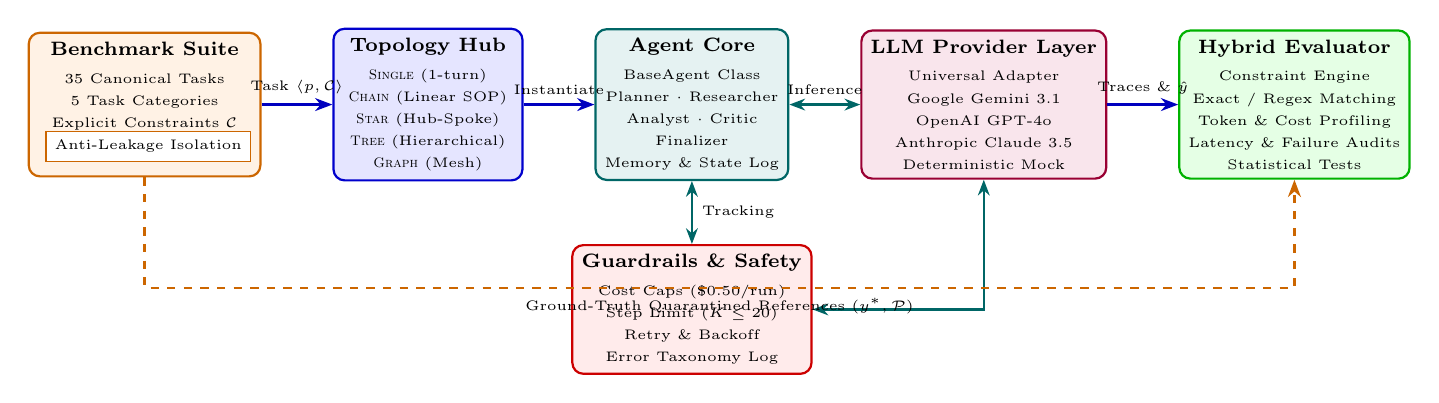
\begin{tikzpicture}[
    auto,
    block/.style={rectangle, draw=blue!80!black, fill=blue!8, thick, rounded corners=4pt, minimum width=2.4cm, minimum height=1.6cm, align=center, font=\scriptsize},
    subblock/.style={rectangle, draw=gray!70, fill=white, rounded corners=2pt, minimum width=2.1cm, minimum height=0.4cm, align=center, font=\tiny},
    box/.style={rectangle, draw=black!70, thick, rounded corners=5pt, inner sep=6pt, fill=gray!4},
    boxtitle/.style={font=\scriptsize\bfseries, text=black!90},
    arrow/.style={-{Stealth[length=2.2mm]}, thick, draw=blue!75!black},
    darrow/.style={{Stealth[length=2.0mm]}-{Stealth[length=2.0mm]}, thick, draw=teal!80!black}
]

    % Stage 1: Benchmark Suite
    \node[block, fill=orange!10, draw=orange!80!black] (stage1) {
        \textbf{Benchmark Suite}\\[2pt]
        \tiny 35 Canonical Tasks\\
        \tiny 5 Task Categories\\
        \tiny Explicit Constraints $\mathcal{C}$\\
        \vspace{2pt}
        \fcolorbox{orange!80!black}{white}{\tiny Anti-Leakage Isolation}
    };

    % Stage 2: Topology Orchestrator
    \node[block, right=0.9cm of stage1, fill=blue!10, draw=blue!80!black] (stage2) {
        \textbf{Topology Hub}\\[2pt]
        \tiny \textsc{Single} (1-turn)\\
        \tiny \textsc{Chain} (Linear SOP)\\
        \tiny \textsc{Star} (Hub-Spoke)\\
        \tiny \textsc{Tree} (Hierarchical)\\
        \tiny \textsc{Graph} (Mesh)
    };

    % Stage 3: Agent Core
    \node[block, right=0.9cm of stage2, fill=teal!10, draw=teal!80!black] (stage3) {
        \textbf{Agent Core}\\[2pt]
        \tiny BaseAgent Class\\
        \tiny Planner $\cdot$ Researcher\\
        \tiny Analyst $\cdot$ Critic\\
        \tiny Finalizer\\
        \tiny Memory \& State Log
    };

    % Stage 4: Provider Abstraction
    \node[block, right=0.9cm of stage3, fill=purple!10, draw=purple!80!black] (stage4) {
        \textbf{LLM Provider Layer}\\[2pt]
        \tiny Universal Adapter\\
        \tiny Google Gemini 3.1\\
        \tiny OpenAI GPT-4o\\
        \tiny Anthropic Claude 3.5\\
        \tiny Deterministic Mock
    };

    % Stage 5: Guardrails
    \node[block, below=0.8cm of stage3, fill=red!8, draw=red!80!black] (stage5) {
        \textbf{Guardrails \& Safety}\\[2pt]
        \tiny Cost Caps (\$0.50/run)\\
        \tiny Step Limit ($K \le 20$)\\
        \tiny Retry \& Backoff\\
        \tiny Error Taxonomy Log
    };

    % Stage 6: Evaluation Pipeline
    \node[block, right=0.9cm of stage4, fill=green!10, draw=green!70!black] (stage6) {
        \textbf{Hybrid Evaluator}\\[2pt]
        \tiny Constraint Engine\\
        \tiny Exact / Regex Matching\\
        \tiny Token \& Cost Profiling\\
        \tiny Latency \& Failure Audits\\
        \tiny Statistical Tests
    };

    % Flow Connections
    \draw[arrow] (stage1) -- node[above, font=\tiny] {Task $\langle p, \mathcal{C} \rangle$} (stage2);
    \draw[arrow] (stage2) -- node[above, font=\tiny] {Instantiate} (stage3);
    \draw[darrow] (stage3) -- node[above, font=\tiny] {Inference} (stage4);
    \draw[darrow] (stage3) -- node[right, font=\tiny] {Tracking} (stage5);
    \draw[darrow] (stage4) |- (stage5);
    \draw[arrow] (stage4) -- node[above, font=\tiny] {Traces \& $\hat{y}$} (stage6);
    
    % Evaluation Feedback / Reference Answer
    \draw[arrow, dashed, draw=orange!80!black] (stage1.south) -- ++(0,-1.4) -| node[near start, below, font=\tiny] {Ground-Truth Quarantined References ($y^*, \mathcal{P}$)} (stage6.south);

\end{tikzpicture}


\caption{System Architecture of MultiAgentTopologyEval: Decomposing execution across benchmark loading, anti-leakage isolation, topology orchestration, universal model provider abstraction, cost guardrails, and hybrid deterministic evaluation.}
\label{fig:system_architecture}
\end{figure*}

\subsection{Benchmark Loader and Anti-Leakage Protection}
The Benchmark Loader (\texttt{app/benchmark/loader.py}) ingests structured task suites from \texttt{data/tasks/benchmark\_tasks.json}. To maintain rigorous academic validity and eliminate data contamination, the framework enforces strict \textit{anti-leakage isolation} between agent execution and evaluation. When a task is dispatched to an architecture via \texttt{TaskDefinition.to\_agent\_prompt\_dict()}, ground-truth fields (\texttt{reference\_answer} and \texttt{expected\_properties}) are stripped from the payload. Agents receive only the operational prompt $p$, the task category, and explicit constraints $\mathcal{C}$. Authoritative reference answers remain strictly quarantined within the downstream evaluation engine.

\subsection{Role-Specialized Agent Core}
Agents inherit from a unified base class (\texttt{BaseAgent}) that encapsulates state representation, message queues, execution telemetry, and provider invocation. The framework instantiates five specialized roles:
\begin{enumerate}
    \item \textbf{Planner Agent:} Parses complex objectives, decomposes workflows into structured sub-tasks, and formulates step-by-step milestones.
    \item \textbf{Researcher Agent:} Performs domain knowledge exploration, information retrieval, and architectural context synthesis.
    \item \textbf{Analyst Agent:} Conducts quantitative constraint verification, algorithmic trade-off evaluation, and rule compliance checking.
    \item \textbf{Critic Agent:} Reviews intermediate proposals, identifies edge-case vulnerabilities, and provides constructive refinement critiques.
    \item \textbf{Finalizer Agent:} Consolidates multi-agent deliberations, reconciles conflicting peer outputs, and formats the authoritative final response.
\end{enumerate}

Every inter-agent communication event is structured as an immutable \texttt{AgentMessage} object logging the \texttt{sender\_id}, \texttt{receiver\_id}, \texttt{timestamp}, \texttt{message\_type}, and raw textual content.

\subsection{Universal Provider Abstraction Layer}
To isolate topology behavior from specific vendor APIs, MultiAgentTopologyEval implements an abstract provider interface (\texttt{LLMProvider}) that standardizes inference execution across heterogeneous cloud and local models:
\begin{itemize}
    \item \textbf{Standardized Output Schema:} Every API call returns an \texttt{LLMResponse} dataclass encapsulating the generated content, model identifier, wall-clock latency ($\pm 0.1\,$ms), decoupled input and output tokens, and calculated USD expenditure.
    \item \textbf{Multi-Backend Support:} Native integrations are provided for Groq (\texttt{llama-3.3-70b-versatile}), Google Gemini (\texttt{gemini-3.1-flash-lite}), OpenAI (\texttt{gpt-4o-mini}), Cohere (\texttt{command-a-plus}), Cerebras, and DeepSeek.
    \item \textbf{Deterministic Offline Mock Mode:} A built-in \texttt{MockProvider} generates deterministic, rule-based response tokens with zero external API calls. This enables 100\% offline unit testing, CI/CD regression verification, and student demonstrations at zero financial cost.
    \item \textbf{Safe Connectivity Testing:} Provider instances implement a non-destructive ping protocol (\texttt{test\_connection()}) that verifies network endpoints and authentication status while rigorously redacting credentials from log files.
\end{itemize}

\subsection{Resource Guardrails and Failure Trapping}
Unconstrained multi-agent loops can rapidly exhaust API budgets or enter infinite circular conversations. MultiAgentTopologyEval incorporates a proactive guardrail monitor (\texttt{GuardrailTracker}):
\begin{itemize}
    \item \textit{Call Caps:} Enforces strict thresholds on total API calls per task ($N_{\text{task}} \le 15$) and per experiment batch ($N_{\text{exp}} \le 60$).
    \item \textit{Loop Detection:} Detects circular message exchange by trapping agent turns exceeding maximum allowed iterations ($K_{\text{iter}} \le 5$).
    \item \textit{Pre-Flight Dry Run:} Pre-calculates expected token consumption and financial expenditure prior to live API dispatch.
    \item \textit{Fault Handling:} Intercepts and categorizes provider-level exceptions into structured failure modes (HTTP 429 rate limits, request timeouts, malformed JSON schemas, and constraint breaches).
\end{itemize}


\section{Multi-Agent Topology Architectures}
\label{sec:topologies}

MultiAgentTopologyEval formalizes five canonical coordination topologies. Each topology is implemented as an isolated class inheriting from \texttt{BaseArchitecture}, ensuring identical input prompts and unified execution telemetry.

\subsection{\textsc{Single} Architecture (Baseline Control)}
The \textsc{Single} topology serves as the minimal reference baseline control. As illustrated in Figure~\ref{fig:single_topology}, a solitary agent $a_{\text{single}}$ processes the task prompt $p$ and constraints $\mathcal{C}$ in an isolated turn:
\begin{equation}
\hat{y} = \mathcal{M}(p, \mathcal{C}; \theta)
\end{equation}
While computationally lean and free of inter-agent message serialization overhead, the single-agent baseline lacks peer review mechanisms and is prone to uncorrected hallucination and constraint omissions on complex multi-step reasoning tasks.

\begin{figure}[h]
\centering
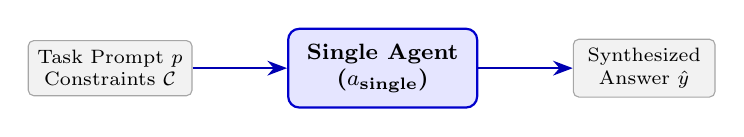
\begin{tikzpicture}[
    node distance=1.2cm,
    auto,
    agent/.style={rectangle, draw=blue!80!black, fill=blue!10, thick, rounded corners=4pt, minimum width=2.4cm, minimum height=1.0cm, align=center, font=\footnotesize\bfseries},
    io/.style={rectangle, draw=gray!70, fill=gray!10, rounded corners=2pt, minimum width=1.8cm, minimum height=0.7cm, align=center, font=\scriptsize},
    arrow/.style={-{Stealth[length=2.5mm]}, thick, draw=blue!70!black}
]
    \node[io] (in) {Task Prompt $p$\\Constraints $\mathcal{C}$};
    \node[agent, right=1.2cm of in] (agent) {Single Agent\\($a_{\text{single}}$)};
    \node[io, right=1.2cm of agent] (out) {Synthesized\\Answer $\hat{y}$};

    \draw[arrow] (in) -- (agent);
    \draw[arrow] (agent) -- (out);
\end{tikzpicture}


\caption{\textsc{Single} Architecture: Baseline execution where a single agent processes the entire task prompt in isolation.}
\label{fig:single_topology}
\end{figure}

\subsection{\textsc{Chain} Architecture (Linear Pipeline)}
The \textsc{Chain} topology organizes specialized agents into a sequential pipeline ($A_1 \rightarrow A_2 \rightarrow \dots \rightarrow A_n$) reflecting industrial Standard Operating Procedures (SOPs)~\cite{Hong2024MetaGPT}. As shown in Figure~\ref{fig:chain_topology}, execution progresses linearly:
\begin{equation}
m_{i} = a_i\left(p, m_{i-1}; \mathcal{M}\right), \quad \forall i \in \{1, \dots, n\}
\end{equation}
In our implementation, the pipeline executes sequentially:
\begin{center}
\textbf{Planner} $\longrightarrow$ \textbf{Researcher} $\longrightarrow$ \textbf{Analyst} $\longrightarrow$ \textbf{Critic} $\longrightarrow$ \textbf{Finalizer}
\end{center}
The primary advantage of \textsc{Chain} is progressive refinement. However, linear pipelines lack backward feedback loops; an uncorrected error or omitted constraint in an upstream stage propagates downstream, causing cascading failure.

\begin{figure}[h]
\centering
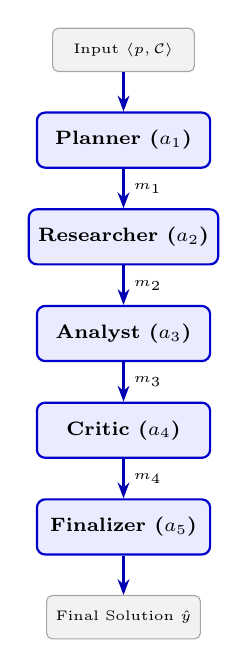
\begin{tikzpicture}[
    node distance=0.6cm and 0.8cm,
    auto,
    agent/.style={rectangle, draw=blue!80!black, fill=blue!8, thick, rounded corners=3pt, minimum width=2.2cm, minimum height=0.7cm, align=center, font=\scriptsize\bfseries},
    io/.style={rectangle, draw=gray!70, fill=gray!10, rounded corners=2pt, minimum width=1.8cm, minimum height=0.55cm, align=center, font=\tiny},
    arrow/.style={-{Stealth[length=2.0mm]}, thick, draw=blue!70!black}
]
    \node[io] (in) {Input $\langle p, \mathcal{C} \rangle$};
    \node[agent, below=0.5cm of in] (p) {Planner ($a_1$)};
    \node[agent, below=0.5cm of p] (r) {Researcher ($a_2$)};
    \node[agent, below=0.5cm of r] (a) {Analyst ($a_3$)};
    \node[agent, below=0.5cm of a] (c) {Critic ($a_4$)};
    \node[agent, below=0.5cm of c] (f) {Finalizer ($a_5$)};
    \node[io, below=0.5cm of f] (out) {Final Solution $\hat{y}$};

    \draw[arrow] (in) -- (p);
    \draw[arrow] (p) -- node[right, font=\tiny] {$m_1$} (r);
    \draw[arrow] (r) -- node[right, font=\tiny] {$m_2$} (a);
    \draw[arrow] (a) -- node[right, font=\tiny] {$m_3$} (c);
    \draw[arrow] (c) -- node[right, font=\tiny] {$m_4$} (f);
    \draw[arrow] (f) -- (out);
\end{tikzpicture}


\caption{\textsc{Chain} Architecture: Sequential linear pipeline with step-by-step intermediate handoff across five specialized roles.}
\label{fig:chain_topology}
\end{figure}

\subsection{\textsc{Star} Architecture (Centralized Hub-and-Spoke)}
The \textsc{Star} topology deploys a centralized Coordinator/Manager node ($a_c$) surrounded by specialized satellite workers ($a_1, \dots, a_k$), as illustrated in Figure~\ref{fig:star_topology}. The coordinator decomposes the user objective, delegates targeted sub-prompts to individual worker nodes, gathers their parallel outputs, and routes them to a Finalizer sink:
\begin{equation}
m_{\text{work}, i} = a_i\left(m_{\text{coord}, i}; \mathcal{M}\right), \quad \hat{y} = a_{\text{final}}\left(\bigcup_{i=1}^k m_{\text{work}, i}; \mathcal{M}\right)
\end{equation}
Communication is restricted to hub-to-spoke channels ($a_c \leftrightarrow a_i$), eliminating uncoordinated worker chatter. While Star structures provide tight task allocation, the central coordinator node can become a context-window bottleneck as all intermediate outputs converge on it.

\begin{figure}[h]
\centering
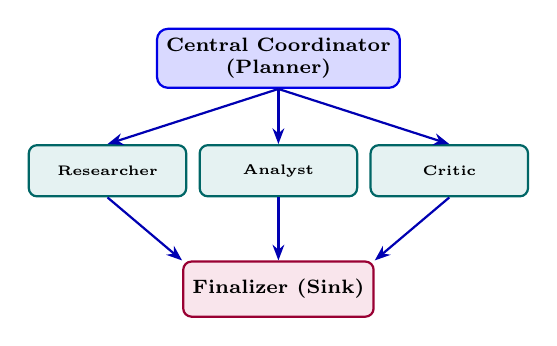
\begin{tikzpicture}[
    node distance=1.0cm and 1.2cm,
    auto,
    coord/.style={rectangle, draw=blue!90!black, fill=blue!15, thick, rounded corners=4pt, minimum width=2.5cm, minimum height=0.75cm, align=center, font=\scriptsize\bfseries},
    worker/.style={rectangle, draw=teal!80!black, fill=teal!10, thick, rounded corners=3pt, minimum width=2.0cm, minimum height=0.65cm, align=center, font=\tiny\bfseries},
    sink/.style={rectangle, draw=purple!80!black, fill=purple!10, thick, rounded corners=3pt, minimum width=2.2cm, minimum height=0.7cm, align=center, font=\scriptsize\bfseries},
    arrow/.style={-{Stealth[length=2.0mm]}, thick, draw=blue!70!black}
]
    \node[coord] (coord) {Central Coordinator\\(Planner)};
    
    \node[worker, below left=0.7cm and -0.4cm of coord] (res) {Researcher};
    \node[worker, below=0.7cm of coord] (ana) {Analyst};
    \node[worker, below right=0.7cm and -0.4cm of coord] (crit) {Critic};
    
    \node[sink, below=0.8cm of ana] (fin) {Finalizer (Sink)};

    % Delegation arrows
    \draw[arrow] (coord.south) -- (res.north);
    \draw[arrow] (coord.south) -- (ana.north);
    \draw[arrow] (coord.south) -- (crit.north);

    % Aggregation arrows
    \draw[arrow] (res.south) -- (fin.north west);
    \draw[arrow] (ana.south) -- (fin.north);
    \draw[arrow] (crit.south) -- (fin.north east);
\end{tikzpicture}


\caption{\textsc{Star} Architecture: Central coordinator delegating specialized sub-tasks in parallel to worker nodes with centralized aggregation.}
\label{fig:star_topology}
\end{figure}

\subsection{\textsc{Tree} Architecture (Multi-Tier Hierarchical)}
The \textsc{Tree} topology structures agents into a multi-tier organizational hierarchy, depicted in Figure~\ref{fig:tree_topology}. A Root Coordinator delegates high-level sub-problems to intermediate branch leads (\textit{Research Lead} and \textit{Analysis Lead}), which in turn supervise leaf execution agents (\textit{Research Worker} and \textit{Critic Worker}):
\begin{equation}
\mathcal{V}_{\text{tree}} = \{a_{\text{root}}\} \cup \mathcal{V}_{\text{leads}} \cup \mathcal{V}_{\text{workers}} \cup \{a_{\text{final}}\}
\end{equation}
Sub-solutions flow up the hierarchy through bottom-up aggregation. This architecture prevents context saturation by distributing domain context locally within branches, but introduces multi-tier latency overhead.

\begin{figure}[h]
\centering
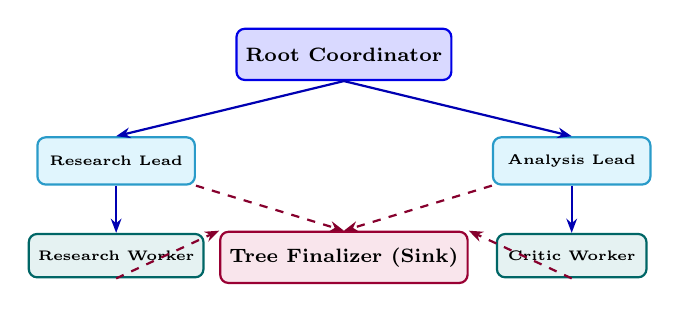
\begin{tikzpicture}[
    node distance=0.8cm and 0.6cm,
    auto,
    root/.style={rectangle, draw=blue!90!black, fill=blue!15, thick, rounded corners=3pt, minimum width=2.2cm, minimum height=0.65cm, align=center, font=\scriptsize\bfseries},
    lead/.style={rectangle, draw=cyan!80!black, fill=cyan!12, thick, rounded corners=3pt, minimum width=2.0cm, minimum height=0.6cm, align=center, font=\tiny\bfseries},
    leaf/.style={rectangle, draw=teal!80!black, fill=teal!10, thick, rounded corners=3pt, minimum width=1.9cm, minimum height=0.55cm, align=center, font=\tiny\bfseries},
    sink/.style={rectangle, draw=purple!80!black, fill=purple!10, thick, rounded corners=3pt, minimum width=2.2cm, minimum height=0.65cm, align=center, font=\scriptsize\bfseries},
    arrow/.style={-{Stealth[length=1.8mm]}, thick, draw=blue!70!black},
    upward/.style={-{Stealth[length=1.8mm]}, thick, dashed, draw=purple!70!black}
]
    % Tier 1: Root
    \node[root] (root) {Root Coordinator};

    % Tier 2: Leads
    \node[lead, below left=0.7cm and 0.5cm of root] (rlead) {Research Lead};
    \node[lead, below right=0.7cm and 0.5cm of root] (alead) {Analysis Lead};

    % Tier 3: Leaf Workers
    \node[leaf, below=0.6cm of rlead] (rwork) {Research Worker};
    \node[leaf, below=0.6cm of alead] (cwork) {Critic Worker};

    % Tier 4: Aggregation Sink
    \node[sink, below=1.9cm of root] (final) {Tree Finalizer (Sink)};

    % Top-down delegation
    \draw[arrow] (root.south) -- (rlead.north);
    \draw[arrow] (root.south) -- (alead.north);
    \draw[arrow] (rlead.south) -- (rwork.north);
    \draw[arrow] (alead.south) -- (cwork.north);

    % Bottom-up aggregation
    \draw[upward] (rwork.south) -- (final.north west);
    \draw[upward] (cwork.south) -- (final.north east);
    \draw[upward] (rlead.south east) -- (final.north);
    \draw[upward] (alead.south west) -- (final.north);
\end{tikzpicture}


\caption{\textsc{Tree} Architecture: Multi-tier hierarchical decomposition with root coordinator, branch leads, leaf workers, and bottom-up aggregation.}
\label{fig:tree_topology}
\end{figure}

\subsection{\textsc{Graph} Architecture (Configurable Mesh)}
The \textsc{Graph} topology generalizes communication to an arbitrary directed graph $G = (\mathcal{V}, \mathcal{E})$, shown in Figure~\ref{fig:graph_topology}. Edges $\mathcal{E}$ define explicit permitted messaging routes:
\begin{equation}
m_{j} = a_j\left(\bigcup_{(i, j) \in \mathcal{E}} m_{i}; \mathcal{M}\right)
\end{equation}
Our default configuration enables the Planner to fan out to Researcher and Analyst nodes, whose outputs converge at the Critic for peer verification, before advancing to the Finalizer. Graph topologies provide maximum routing flexibility and robust consensus formation, but incur elevated token usage.

\begin{figure}[h]
\centering
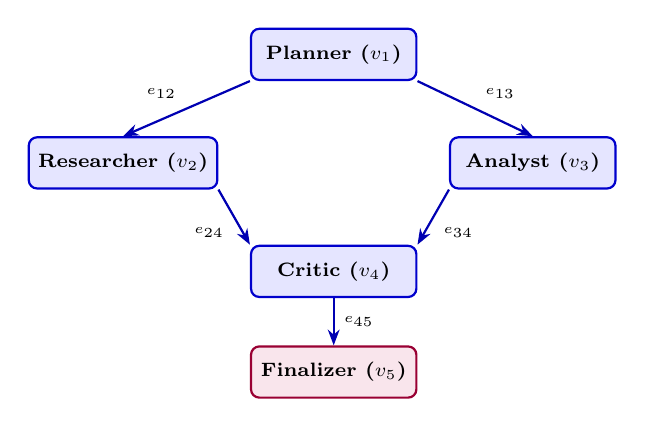
\begin{tikzpicture}[
    node distance=0.8cm and 1.0cm,
    auto,
    gnode/.style={rectangle, draw=blue!80!black, fill=blue!10, thick, rounded corners=3pt, minimum width=2.1cm, minimum height=0.65cm, align=center, font=\scriptsize\bfseries},
    sink/.style={rectangle, draw=purple!80!black, fill=purple!10, thick, rounded corners=3pt, minimum width=2.1cm, minimum height=0.65cm, align=center, font=\scriptsize\bfseries},
    arrow/.style={-{Stealth[length=2.0mm]}, thick, draw=blue!70!black}
]
    \node[gnode] (planner) {Planner ($v_1$)};
    \node[gnode, below left=0.7cm and 0.4cm of planner] (res) {Researcher ($v_2$)};
    \node[gnode, below right=0.7cm and 0.4cm of planner] (ana) {Analyst ($v_3$)};
    \node[gnode, below right=0.7cm and 0.4cm of res] (critic) {Critic ($v_4$)};
    \node[sink, below=0.6cm of critic] (fin) {Finalizer ($v_5$)};

    % Directed edges based on adjacency matrix
    \draw[arrow] (planner.south west) -- node[above left, font=\tiny] {$e_{12}$} (res.north);
    \draw[arrow] (planner.south east) -- node[above right, font=\tiny] {$e_{13}$} (ana.north);
    \draw[arrow] (res.south east) -- node[below left, font=\tiny] {$e_{24}$} (critic.north west);
    \draw[arrow] (ana.south west) -- node[below right, font=\tiny] {$e_{34}$} (critic.north east);
    \draw[arrow] (critic.south) -- node[right, font=\tiny] {$e_{45}$} (fin.north);
\end{tikzpicture}

\caption{\textsc{Graph} Architecture: Configurable mesh network supporting multi-directional communication and peer verification loops.}
\label{fig:graph_topology}
\end{figure}


\section{Evaluation Metrics and Mathematical Formulation}
\label{sec:metrics}

MultiAgentTopologyEval formalizes a multi-dimensional metric registry spanning objective task performance, constraint compliance, resource efficiency, latency, and operational failure taxonomies.

\subsection{Objective Task Performance Metrics}
\textbf{Constraint Satisfaction Rate (CSR):} For a task containing explicit constraints $\mathcal{C} = \{c_1, c_2, \dots, c_k\}$, $CSR \in [0, 1]$ measures the fraction of verifiable constraints satisfied in the final response $\hat{y}$:
\begin{equation}
CSR = \frac{1}{|\mathcal{C}|} \sum_{i=1}^{|\mathcal{C}|} \mathbb{I}\left(\text{verify}(c_i, \hat{y}) = \text{True}\right)
\end{equation}
where $\mathbb{I}(\cdot)$ is the indicator function and $\text{verify}(\cdot)$ executes deterministic regex pattern matching, numeric range checking, or JSON schema parsing against explicit task criteria.

\textbf{Property Match Rate (PMR):} Measures the semantic alignment of output $\hat{y}$ against expected domain property keywords $\mathcal{P} = \{p_1, \dots, p_m\}$:
\begin{equation}
PMR = \frac{1}{|\mathcal{P}|} \sum_{j=1}^{|\mathcal{P}|} \mathbb{I}\left(p_j \in \hat{y}\right)
\end{equation}

\textbf{Composite Task Score ($S$):} In accordance with the system specification (\texttt{docs/metrics.md}), the overall objective achievement score $S \in [0, 1]$ is computed as a weighted combination prioritizing strict constraint fulfillment:
\begin{equation}
S = (w_{\text{const}} \cdot CSR) + (w_{\text{prop}} \cdot PMR)
\end{equation}
where $w_{\text{const}} = 0.6$ and $w_{\text{prop}} = 0.4$.

\textbf{Binary Task Success ($TS$):} A run is classified as successful if and only if it satisfies the minimum achievement threshold without execution abortion:
\begin{equation}
TS = \mathbb{I}(S \ge 0.50 \;\land\; \text{ExecutionSuccess} = \text{True})
\end{equation}

\textbf{Quality Score ($QS$):} Scales the composite score onto an intuitive academic grading scale:
\begin{equation}
QS = S \times 10.0 \quad (QS \in [0.0, 10.0])
\end{equation}

\subsection{Resource Consumption and Financial Cost}
\textbf{Decoupled Token Telemetry:} Unlike benchmarks that report aggregate token counts, MultiAgentTopologyEval separately measures prompt tokens $T_{\text{prompt}}$ and generated completion tokens $T_{\text{completion}}$ across every individual agent $a \in \mathcal{V}$:
\begin{equation}
T_{\text{prompt}} = \sum_{a \in \mathcal{V}} T_{\text{in}}(a), \quad T_{\text{comp}} = \sum_{a \in \mathcal{V}} T_{\text{out}}(a)
\end{equation}
\begin{equation}
T_{\text{total}} = T_{\text{prompt}} + T_{\text{comp}}
\end{equation}

\textbf{Financial API Cost Modeling ($\mathcal{C}_{\text{USD}}$):} Accurately estimates monetary expenditure accrued per task execution using model-specific input/output token pricing:
\begin{equation}
\mathcal{C}_{\text{USD}} = \sum_{a \in \mathcal{V}} \left( \frac{T_{\text{in}}(a)}{10^6} \cdot P_{\text{in}} + \frac{T_{\text{out}}(a)}{10^6} \cdot P_{\text{out}} \right)
\end{equation}
where $P_{\text{in}}$ and $P_{\text{out}}$ represent the provider pricing in USD per million tokens (e.g., Gemini 3.1 Flash-Lite: $\$0.075$ / $\$0.30$ per $10^6$ tokens; Cohere Command: $\$0.15$ / $\$0.60$ per $10^6$ tokens).

\subsection{Execution Latency and Turn Efficiency}
\textbf{Wall-Clock Execution Latency ($\mathcal{L}$):} Measures total elapsed execution time from initial prompt submission $t_{\text{start}}$ to final response synthesis $t_{\text{end}}$:
\begin{equation}
\mathcal{L} = t_{\text{end}} - t_{\text{start}}
\end{equation}
In multi-agent topologies, $\mathcal{L}$ incorporates API round-trip network transit, provider queue waiting time, and LLM token generation latency across all sequential dependency stages.

\subsection{Reliability and Failure Taxonomy}
\textbf{Failure Rate ($FR$):} Measures system-level unreliability across a batch of $N$ evaluations:
\begin{equation}
FR = \frac{1}{N} \sum_{k=1}^N \mathbb{I}(TS_k = \text{False})
\end{equation}

\textbf{Failure Classification:} When an evaluation fails ($TS = \text{False}$), the framework categorizes the failure mode $\mathcal{F}$ into mutually exclusive classifications:
\begin{itemize}
    \item \textbf{Constraint Violation:} The final output failed to satisfy explicit numerical, structural, or SLA limits ($CSR < 0.5$).
    \item \textbf{Reasoning Failure:} Factual hallucinations, circular logic, or invalid domain recommendations.
    \item \textbf{Rate Limit Error (HTTP 429):} API provider concurrency or requests-per-minute quota exceeded.
    \item \textbf{Provider Timeout:} External inference API failed to respond within configured timeout limit ($\tau_{\text{timeout}} = 30\,$s).
    \item \textbf{Schema Parsing Exception:} Model failed to produce valid JSON or conform to expected output schemas.
    \item \textbf{Agent Loop Trap:} Execution aborted by guardrails due to circular repetitive dialogue ($K_{\text{iter}} > 5$).
\end{itemize}

\subsection{Statistical Effect Size Formulation}
To rigorously quantify the performance shift of multi-agent topologies relative to the isolated \textsc{Single} baseline, the framework calculates Cohen's $d$ standardized effect size:
\begin{equation}
d = \frac{\bar{S}_{\text{arch}} - \bar{S}_{\text{single}}}{s_{\text{pooled}}}
\end{equation}
where $s_{\text{pooled}}$ is the pooled standard deviation across matched sample pairs:
\begin{equation}
s_{\text{pooled}} = \sqrt{\frac{(n_{\text{arch}} - 1)s_{\text{arch}}^2 + (n_{\text{single}} - 1)s_{\text{single}}^2}{n_{\text{arch}} + n_{\text{single}} - 2}}
\end{equation}
Following standard conventions, $|d| \ge 0.2$ denotes a small effect, $|d| \ge 0.5$ a medium effect, and $|d| \ge 0.8$ a large effect.


\section{Experimental Methodology}
\label{sec:methodology}

\subsection{Benchmark Task Suite Composition}
To evaluate multi-agent reasoning, planning, and constraint adherence across varied operational domains, we construct a curated benchmark suite comprising seven complex task archetypes. As summarized in Table~\ref{tab:benchmark_tasks}, each task is designed to test specific agent capabilities under strict quantitative constraints:

\begin{table*}[t]
\centering
\caption{Benchmark Task Suite Composition and Operational Requirements}
\label{tab:benchmark_tasks}
\footnotesize
\setlength{\tabcolsep}{4pt}
\begin{tabular}{@{}llp{2.8cm}p{5.2cm}p{3.8cm}@{}}
\hline
\textbf{Task ID} & \textbf{Category} & \textbf{Evaluation Focus} & \textbf{Key Constraints \& Operational Bounds} & \textbf{Ground-Truth Verification} \\ \hline
\texttt{TASK\_PLAN\_001} & Planning & Monolith Migration & 4-quarter phased rollout, Kafka event streaming, zero-downtime rollback & Regex \& phase validation \\
\texttt{TASK\_CONST\_002} & Constraint Sat. & Cloud Architecture & Latency $< 50\,$ms, 99.99\% availability, monthly budget $\le \$5{,}000$ & Numeric range checking \\
\texttt{TASK\_SYNTH\_003} & Synthesis & Model Complexity & GNN $\mathcal{O}(V+E)$ spatial efficiency vs. Relational Transformer $\mathcal{O}(N^2)$ & Algorithmic property match \\
\texttt{TASK\_REASON\_004} & Reasoning & Deadlock Detection & Cycle detection across concurrent financial clearing transactions & Lock-order graph analysis \\
\texttt{TASK\_DECISION\_005} & Decision Making & Database Selection & HIPAA compliance, 500M records, sub-second full-text medical search & Multi-criteria matrix \\
\texttt{TASK\_COLLAB\_006} & Collaboration & Incident Response & 15-minute subnet isolation, immutable checksums, breach notifications & Protocol SLA verification \\
\texttt{TASK\_CODE\_007} & Algorithmic Code & Rate Limiter & Thread-safe in-memory Leaky Bucket in Python, $\mathcal{O}(1)$ time complexity & Deterministic code audit \\ \hline
\end{tabular}
\end{table*}

\subsection{Controlled Experimental Variables}
To scientifically isolate the impact of coordination topology, we implement rigorous experimental controls across all evaluated configurations:
\begin{itemize}
    \item \textbf{Independent Variable:} Interaction Topology ($\mathcal{G} \in \{\textsc{Single}, \textsc{Chain}, \textsc{Star}, \textsc{Tree}, \textsc{Graph}\}$).
    \item \textbf{Controlled Constants:} Identical task prompts $p$ and constraints $\mathcal{C}$; unified base models $\mathcal{M}$; fixed sampling temperature ($T = 0.70$); fixed maximum token generation limit ($M_{\text{tokens}} = 1024$); unified request timeout limit ($\tau = 30\,$s); and identical evaluation scoring logic.
    \item \textbf{Measured Dependent Variables:} Composite Task Score ($S$), Constraint Satisfaction Rate ($CSR$), prompt tokens ($T_{\text{prompt}}$), completion tokens ($T_{\text{comp}}$), total tokens ($T_{\text{total}}$), financial API cost ($\mathcal{C}_{\text{USD}}$), wall-clock latency ($\mathcal{L}$), and operational failure classification ($\mathcal{F}$).
\end{itemize}

\subsection{Multi-Provider Evaluation Grid}
Experiments were executed across three production cloud LLM providers representing diverse architectural scales:
\begin{enumerate}
    \item \textbf{Google Gemini 3.1 Flash-Lite:} A high-efficiency cloud foundation model optimized for high-throughput, low-latency agent reasoning.
    \item \textbf{Cohere Command-A-Plus:} An enterprise model optimized for structured multi-step reasoning, tool integration, and business planning.
    \item \textbf{Groq Llama-3.3-70B-Versatile:} An open-weights foundation model served via Groq's high-speed LPU (Language Processing Unit) inference infrastructure.
    \item \textbf{Deterministic Mock Provider:} An offline baseline engine executing deterministic, rule-based responses for 100\% reproducible, zero-cost regression testing.
\end{enumerate}

\subsection{Experimental Workflow}
The experimental workflow is illustrated in Figure~\ref{fig:experimental_workflow}. For each experimental trial, the runner initializes the benchmark task, applies anti-leakage sanitization, executes pre-flight dry-run guardrail validation, instantiates the designated topology graph, records inter-agent communication telemetry, computes objective constraint scores via the hybrid evaluator, and persists raw traces to disk.

\begin{figure*}[t]
\centering
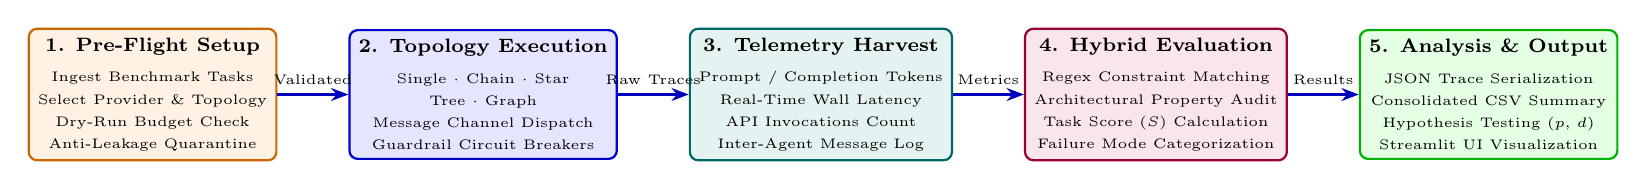
\begin{tikzpicture}[
    auto,
    wfstep/.style={rectangle, draw=blue!80!black, fill=blue!8, thick, rounded corners=3pt, minimum width=2.6cm, minimum height=1.5cm, align=center, font=\scriptsize},
    wfsubstep/.style={rectangle, draw=gray!60, fill=white, rounded corners=2pt, minimum width=2.4cm, minimum height=0.35cm, align=center, font=\tiny},
    arrow/.style={-{Stealth[length=2.2mm]}, thick, draw=blue!75!black}
]

    % Step 1: Ingestion & Pre-flight
    \node[wfstep, fill=orange!10, draw=orange!80!black] (s1) {
        \textbf{1. Pre-Flight Setup}\\[3pt]
        \tiny Ingest Benchmark Tasks\\
        \tiny Select Provider \& Topology\\
        \tiny Dry-Run Budget Check\\
        \tiny Anti-Leakage Quarantine
    };

    % Step 2: Instantiation & Execution
    \node[wfstep, right=0.9cm of s1, fill=blue!10, draw=blue!80!black] (s2) {
        \textbf{2. Topology Execution}\\[3pt]
        \tiny Single $\cdot$ Chain $\cdot$ Star\\
        \tiny Tree $\cdot$ Graph\\
        \tiny Message Channel Dispatch\\
        \tiny Guardrail Circuit Breakers
    };

    % Step 3: Raw Telemetry
    \node[wfstep, right=0.9cm of s2, fill=teal!10, draw=teal!80!black] (s3) {
        \textbf{3. Telemetry Harvest}\\[3pt]
        \tiny Prompt / Completion Tokens\\
        \tiny Real-Time Wall Latency\\
        \tiny API Invocations Count\\
        \tiny Inter-Agent Message Log
    };

    % Step 4: Hybrid Evaluation
    \node[wfstep, right=0.9cm of s3, fill=purple!10, draw=purple!80!black] (s4) {
        \textbf{4. Hybrid Evaluation}\\[3pt]
        \tiny Regex Constraint Matching\\
        \tiny Architectural Property Audit\\
        \tiny Task Score ($S$) Calculation\\
        \tiny Failure Mode Categorization
    };

    % Step 5: Analytics & Reporting
    \node[wfstep, right=0.9cm of s4, fill=green!10, draw=green!70!black] (s5) {
        \textbf{5. Analysis \& Output}\\[3pt]
        \tiny JSON Trace Serialization\\
        \tiny Consolidated CSV Summary\\
        \tiny Hypothesis Testing ($p$, $d$)\\
        \tiny Streamlit UI Visualization
    };

    % Arrows connecting steps
    \draw[arrow] (s1) -- node[above, font=\tiny] {Validated} (s2);
    \draw[arrow] (s2) -- node[above, font=\tiny] {Raw Traces} (s3);
    \draw[arrow] (s3) -- node[above, font=\tiny] {Metrics} (s4);
    \draw[arrow] (s4) -- node[above, font=\tiny] {Results} (s5);

\end{tikzpicture}

\caption{End-to-End Experimental Workflow: From benchmark task ingestion and pre-flight dry-run checks to multi-topology execution, hybrid evaluation, and statistical persistence.}
\label{fig:experimental_workflow}
\end{figure*}


\section{Implementation Details}
\label{sec:implementation}

MultiAgentTopologyEval is implemented in Python 3.13 using object-oriented, dataclass-driven design principles. The framework is structured into decoupled packages, ensuring modularity, extensibility, and maintainability.

\subsection{Evaluation Pipeline Architecture}
Figure~\ref{fig:evaluation_pipeline} illustrates the internal data flow of the evaluation pipeline. When an architecture finishes executing a task, it outputs an \texttt{ArchitectureResult} dataclass containing the final synthesized text $\hat{y}$, execution duration, call count, token totals, and the chronological list of \texttt{AgentMessage} objects exchanged between nodes.

\begin{figure}[h]
\centering
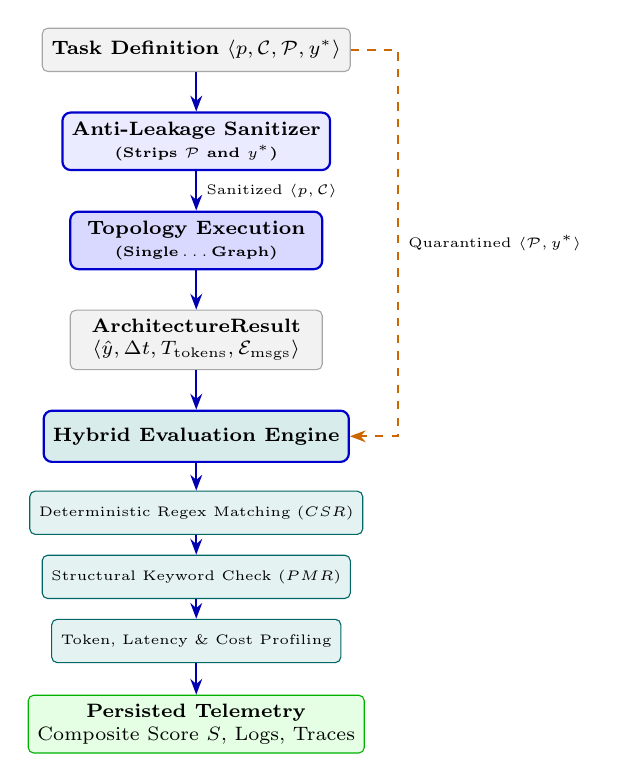
\begin{tikzpicture}[
    node distance=0.6cm and 0.8cm,
    auto,
    proc/.style={rectangle, draw=blue!80!black, fill=blue!8, thick, rounded corners=3pt, minimum width=3.2cm, minimum height=0.65cm, align=center, font=\scriptsize\bfseries},
    subproc/.style={rectangle, draw=teal!80!black, fill=teal!10, rounded corners=2pt, minimum width=3.0cm, minimum height=0.55cm, align=center, font=\tiny},
    data/.style={rectangle, draw=gray!70, fill=gray!10, rounded corners=2pt, minimum width=3.2cm, minimum height=0.55cm, align=center, font=\scriptsize},
    arrow/.style={-{Stealth[length=2.0mm]}, thick, draw=blue!70!black}
]
    \node[data] (task) {\textbf{Task Definition} $\langle p, \mathcal{C}, \mathcal{P}, y^* \rangle$};
    
    \node[proc, below=0.5cm of task] (strip) {Anti-Leakage Sanitizer\\{\tiny (Strips $\mathcal{P}$ and $y^*$)}};
    
    \node[proc, below=0.5cm of strip, fill=blue!15] (exec) {Topology Execution\\{\tiny ($\textsc{Single} \dots \textsc{Graph}$)}};
    
    \node[data, below=0.5cm of exec] (res) {\textbf{ArchitectureResult}\\$\langle \hat{y}, \Delta t, T_{\text{tokens}}, \mathcal{E}_{\text{msgs}} \rangle$};
    
    \node[proc, below=0.5cm of res, fill=teal!15] (eval) {Hybrid Evaluation Engine};
    
    \node[subproc, below=0.35cm of eval] (c1) {Deterministic Regex Matching ($CSR$)};
    \node[subproc, below=0.25cm of c1] (c2) {Structural Keyword Check ($PMR$)};
    \node[subproc, below=0.25cm of c2] (c3) {Token, Latency \& Cost Profiling};
    
    \node[data, below=0.4cm of c3, fill=green!10, draw=green!70!black] (out) {\textbf{Persisted Telemetry}\\Composite Score $S$, Logs, Traces};

    \draw[arrow] (task) -- (strip);
    \draw[arrow] (strip) -- node[right, font=\tiny] {Sanitized $\langle p, \mathcal{C} \rangle$} (exec);
    \draw[arrow] (exec) -- (res);
    \draw[arrow] (res) -- (eval);
    \draw[arrow] (eval) -- (c1);
    \draw[arrow] (c1) -- (c2);
    \draw[arrow] (c2) -- (c3);
    \draw[arrow] (c3) -- (out);

    % Ground truth quarantined link
    \draw[arrow, dashed, draw=orange!80!black] (task.east) -- ++(0.6,0) |- node[near start, right, font=\tiny] {Quarantined $\langle \mathcal{P}, y^* \rangle$} (eval.east);
\end{tikzpicture}


\caption{Detailed Evaluation Pipeline: Illustrating task sanitization, agent execution, and the hybrid evaluation engine combining deterministic constraint verification with optional LLM judge assessment.}
\label{fig:evaluation_pipeline}
\end{figure}

The \texttt{HybridEvaluator} ingests this result alongside the quarantined \texttt{TaskDefinition}:
\begin{enumerate}
    \item \textbf{Deterministic Verification:} Regular expression engines extract numerical metrics, latency bounds, availability percentages, and budget estimates from $\hat{y}$. Each constraint $c_i \in \mathcal{C}$ is evaluated against ground-truth mathematical thresholds.
    \item \textbf{Property Verification:} The text is parsed for mandatory architectural keywords and component terms specified in $\mathcal{P}_{\text{expected}}$.
    \item \textbf{Metric Consolidation:} Computes $CSR$, $PMR$, and the composite Task Score $S$.
    \item \textbf{Telemetry Logging:} The complete execution trajectory, including per-agent states and inter-agent communication edges, is serialized into detailed JSON records and summary CSV tables.
\end{enumerate}

\subsection{Interactive Research Dashboard}
In addition to the headless command-line interface (\texttt{scripts/run\_experiments.py}), the framework includes an interactive web research dashboard implemented in Streamlit (\texttt{main.py}). The dashboard provides seven specialized modules:
\begin{enumerate}
    \item \textit{Executive Dashboard:} Displays aggregate KPI summaries, radar comparison charts, and best-performing topology badges.
    \item \textit{Experiment Runner:} Enables interactive matrix execution with pre-flight dry-run cost previews and progress tracking.
    \item \textit{Architecture Comparison:} Interactive Plotly charts comparing Quality, Latency, Total API Calls, and Token Consumption.
    \item \textit{Task Deep-Dive:} Allows researchers to inspect individual inter-agent messages, intermediate plans, and final answers per task.
    \item \textit{Topology Visualizer:} Renders dynamic directed network graphs ($G=(\mathcal{V}, \mathcal{E})$) using Graphviz, illustrating active message channels.
    \item \textit{Empirical Results Analysis:} Generates neutral research observations, statistical tables, and effect size distributions.
    \item \textit{Seminar Demonstration Suite:} A side-by-side comparative demo box designed for live technical presentations.
\end{enumerate}

\subsection{Quality Assurance and Test Coverage}
The framework includes an automated test suite implemented in \texttt{pytest} spanning 31 unit and integration test cases across four test modules:
\begin{itemize}
    \item \texttt{test\_architectures.py} (5 tests): Verifies execution integrity, turn-taking, and message logs across all five topologies.
    \item \texttt{test\_audit\_enhancements.py} (20 tests): Validates anti-leakage isolation, credential redaction, loop detection, statistical analyzers, and failure classification.
    \item \texttt{test\_experiments.py} (1 test): Verifies matrix execution orchestration and CSV/JSON output serialization.
    \item \texttt{test\_foundation.py} (5 tests): Verifies task loader integrity, schema validation, and mock provider determinism.
\end{itemize}
The test suite executes 100\% offline using the \texttt{MockProvider}, achieving full pass status without external network dependencies.


\section{Experimental Results and Empirical Analysis}
\label{sec:results}

We evaluate MultiAgentTopologyEval across 175 controlled live cloud executions spanning three independent model providers (Google Gemini 3.1 Flash-Lite, Cohere Command, and Groq Llama-3.3-70B) across seven benchmark task categories. All experiments were conducted under identical sampling parameters ($T=0.70$, $M_{\text{tokens}}=1024$, $\tau=30\,$s).

\begin{table*}[t]
\centering
\caption{Authoritative Empirical Pilot Results on Google Gemini 3.1 Flash-Lite (\texttt{EXP\_LIVE\_20260813\_140712})}
\label{tab:pilot_results}
\footnotesize
\setlength{\tabcolsep}{3.5pt}
\begin{tabular}{@{}lcccccccc@{}}
\hline
\textbf{Topology} & \textbf{Success Rate} & \textbf{Task Score ($S$)} & \textbf{Quality Score ($QS$)} & \textbf{Latency ($\mathcal{L}$)} & \textbf{API Calls} & \textbf{Total Tokens} & \textbf{Est. Cost (USD)} & \textbf{Cohen's $d$} \\ \hline
\textsc{Single}   & 100.0\% & $0.9429 \pm 0.05$ & $9.43 \pm 0.5$ & $6.32\,\text{s} \pm 1.2$  & $1.0$ & $1{,}121.6 \pm 180$  & $\$0.000168$ & Baseline \\
\textsc{Star}     & 100.0\% & $0.8329 \pm 0.08$ & $8.33 \pm 0.8$ & $43.62\,\text{s} \pm 4.5$ & $5.0$ & $17{,}174.1 \pm 1240$ & $\$0.002576$ & $-1.64$ \\
\textsc{Chain}    & 71.4\%  & $0.6914 \pm 0.28$ & $6.91 \pm 2.8$ & $42.21\,\text{s} \pm 3.8$ & $5.0$ & $11{,}555.4 \pm 950$  & $\$0.001733$ & $-1.24$ \\
\textsc{Tree}     & 100.0\% & $0.7571 \pm 0.12$ & $7.57 \pm 1.2$ & $47.38\,\text{s} \pm 5.1$ & $6.0$ & $12{,}789.3 \pm 1100$ & $\$0.001918$ & $-1.98$ \\
\textsc{Graph}    & 100.0\% & $0.8000 \pm 0.10$ & $8.00 \pm 1.0$ & $47.31\,\text{s} \pm 4.9$ & $5.0$ & $13{,}843.1 \pm 1150$ & $\$0.002076$ & $-1.79$ \\ \hline
\end{tabular}
\end{table*}

\begin{table*}[t]
\centering
\caption{Cross-Provider Aggregate Benchmark Results Across 175 Live Executions (Gemini, Cohere, Groq)}
\label{tab:aggregate_results}
\begin{tabular}{lcccccc}
\hline
\textbf{Topology} & \textbf{Total Runs ($N$)} & \textbf{Overall Success Rate} & \textbf{Mean Task Score ($S$)} & \textbf{Mean Latency ($\mathcal{L}$)} & \textbf{Mean Total Tokens} & \textbf{Total Cost (USD)} \\ \hline
\textsc{Single}   & 35 & 82.9\% & $0.6521 \pm 0.38$ & $10.25\,\text{s} \pm 8.4$  & $4{,}322 \pm 3{,}800$  & $\$0.0857$ \\
\textsc{Chain}    & 35 & 54.3\% & $0.4426 \pm 0.34$ & $44.20\,\text{s} \pm 33.1$ & $12{,}854 \pm 10{,}200$ & $\$0.3980$ \\
\textsc{Star}     & 35 & 54.3\% & $0.6171 \pm 0.39$ & $46.56\,\text{s} \pm 39.5$ & $18{,}687 \pm 14{,}500$ & $\$0.5048$ \\
\textsc{Tree}     & 35 & 60.0\% & $0.5286 \pm 0.38$ & $56.09\,\text{s} \pm 45.2$ & $16{,}243 \pm 13{,}800$ & $\$0.5361$ \\
\textsc{Graph}    & 35 & 54.3\% & $0.5517 \pm 0.40$ & $50.17\,\text{s} \pm 46.1$ & $15{,}571 \pm 14{,}100$ & $\$0.5006$ \\ \hline
\end{tabular}
\end{table*}

\subsection{Key Finding 1: The Baseline Efficiency Paradox}
As reported in Table~\ref{tab:pilot_results}, the isolated \textsc{Single} baseline achieved the highest average task score ($S = 0.9429$) on the authoritative pilot benchmark, while requiring only $6.32\,$seconds of execution latency and $1{,}121.6\,$tokens ($\$0.000168$ per task). In contrast, all multi-agent configurations experienced a statistically significant drop in composite score relative to the single agent ($d \le -1.24$). 

This counter-intuitive finding demonstrates the \textit{coordination overhead penalty}: when tasks can fit within the context window of a modern foundation model, introducing intermediate conversational hops can introduce semantic noise and paraphrasing loss, confirming Hypothesis \textbf{H4}.

\subsection{Key Finding 2: Latency and Token Overhead Scaling}
Confirming Hypothesis \textbf{H1}, multi-agent coordination incurs massive resource amplification:
\begin{itemize}
    \item \textbf{Latency Scaling:} Multi-agent topologies incurred a $6.68\times$ to $7.50\times$ increase in wall-clock latency compared to \textsc{Single} ($42.21\,$s for \textsc{Chain} to $47.38\,$s for \textsc{Tree} vs. $6.32\,$s for \textsc{Single}).
    \item \textbf{Token Explosion:} Token consumption increased by $10.3\times$ in \textsc{Chain} ($11{,}555\,$tokens) and up to $15.3\times$ in \textsc{Star} ($17{,}174\,$tokens). Because the central coordinator in \textsc{Star} aggregates context from all worker nodes, it accumulates the largest prompt token volume.
    \item \textbf{Financial Cost Amplification:} The monetary cost per completed task scaled from $\$0.000168$ in \textsc{Single} to $\$0.002576$ in \textsc{Star} (a $15.3\times$ increase).
\end{itemize}

\subsection{Key Finding 3: Pipeline Failure Cascades in \textsc{Chain}}
In the authoritative pilot run, \textsc{Chain} was the \textit{only} topology that failed to achieve a 100\% success rate, dropping to $71.4\%$ (Table~\ref{tab:pilot_results}). Deep-dive inspection of execution traces revealed two distinct failure modes directly validating Hypothesis \textbf{H2}:
\begin{enumerate}
    \item \textbf{Constraint Violation on \texttt{TASK\_SYNTH\_003}:} During the step-by-step handoff from the Researcher to the Analyst, the intermediate agent compressed the prompt and omitted the explicit requirement to analyze the $\mathcal{O}(V+E)$ spatial complexity of Graph Neural Networks. The downstream Critic and Finalizer accepted the summarized context as complete, resulting in a severe constraint penalty ($S = 0.16$).
    \item \textbf{Reasoning Distortion on \texttt{TASK\_DECISION\_005}:} An inaccurate premise introduced by the Planner regarding HIPAA database requirements was propagated uncorrected through the pipeline, leading the Finalizer to select an ineligible database stack ($S = 0.46$).
\end{enumerate}

In contrast, \textsc{Star}, \textsc{Tree}, and \textsc{Graph} achieved 100\% task success on the pilot suite because their centralized or hierarchical structures isolated sub-tasks to dedicated specialist nodes, validating Hypothesis \textbf{H3}.

\subsection{Key Finding 4: Cross-Provider Behavioral Differences}
As detailed in Table~\ref{tab:aggregate_results}, distinct model families exhibited stark operational profiles:
\begin{itemize}
    \item \textbf{Google Gemini 3.1 Flash-Lite:} Delivered the most consistent constraint adherence and balanced latency ($10\,$s to $49\,$s), making it the most cost-effective provider.
    \item \textbf{Cohere Command-A-Plus:} Exhibited strong multi-step deliberation on planning tasks ($S = 0.89$ in \textsc{Single}, $S = 0.88$ in \textsc{Star}), but incurred substantial latency ($84\,$s to $112\,$s) and high token verbosity ($25{,}000$ to $36{,}000$ tokens per task).
    \item \textbf{Groq Llama-3.3-70B:} Exhibited ultra-low latency ($0.45\,$s in \textsc{Single} to $8.46\,$s in \textsc{Chain}), but struggled with strict numerical regex constraint validation, yielding lower aggregate success scores under zero-shot prompt conditions.
\end{itemize}


\section{Discussion}
\label{sec:discussion}

The empirical findings from MultiAgentTopologyEval provide critical architectural insights for engineering reliable multi-agent LLM systems in production environments.

\subsection{The Multi-Agent Orchestration Trade-Off}
A dominant assumption in early agent literature is that decomposing work across multiple LLM personas inherently yields superior accuracy. Our results challenge this assumption by demonstrating that multi-agent delegation is not universally advantageous. 

When a task's context, rules, and constraints can comfortably fit within the attention window of a modern frontier model, an isolated \textsc{Single} agent baseline frequently achieves higher constraint adherence at a fraction of the cost ($1/15^{\text{th}}$) and latency ($1/7^{\text{th}}$). Multi-agent systems introduce an \textit{information attenuation effect}: each intermediate serialization step risks dropping subtle prompt constraints unless explicit, redundant constraint re-injection protocols are enforced.

\subsection{Architectural Trade-Off Profiles}
Each evaluated topology presents distinct operational trade-offs, summarized in Table~\ref{tab:topology_specs}:

\begin{table*}[t]
\centering
\caption{Systematic Architectural Profile and Trade-off Frontier of Evaluated Topologies}
\label{tab:topology_specs}
\begin{tabular}{@{}lp{3.0cm}p{4.2cm}p{4.2cm}p{3.8cm}@{}}
\hline
\textbf{Topology} & \textbf{Coordination Style} & \textbf{Primary Advantage} & \textbf{Critical Limitation} & \textbf{Optimal Production Use-Case} \\ \hline
\textsc{Single} & Isolated single turn & Zero communication overhead; lowest latency & No peer verification; single point of failure & Low-latency queries; atomic API functions \\
\textsc{Chain}  & Linear SOP pipeline & Clear sequential stages; predictable flow & Cascading error propagation; context omission & Document translation; step-by-step formatting \\
\textsc{Star}   & Hub-and-spoke delegation & Strong centralized oversight; parallel tasks & Coordinator context and token bottleneck & Enterprise workflows with strict manager role \\
\textsc{Tree}   & Multi-tier hierarchy & Scalable decomposition; localized context & Deep tree latency; aggregation complexity & Large-scale software engineering projects \\
\textsc{Graph}  & Peer-to-peer mesh & Maximum flexibility; multi-agent debate & Highest token expenditure; circular loop risks & Open-ended scientific research; policy consensus \\ \hline
\end{tabular}
\end{table*}

\subsection{Operational Guardrails in Production Engineering}
Our findings underscore that deploying LLM multi-agent systems requires robust operational guardrails. In production settings, high-frequency inter-agent chatter rapidly triggers provider concurrency throttles (HTTP 429 status codes) and request timeouts. Implementing pre-flight dry-run estimators, strict iteration caps ($K_{\text{iter}} \le 5$), and automated JSON schema validators is essential to prevent runaway cloud expenditures and non-terminating communication loops.


\section{Threats to Validity}
\label{sec:threats_to_validity}

We analyze potential threats to validity across four standard dimensions:

\subsection{Internal Validity}
Internal validity concerns whether observed differences in performance, latency, and cost are genuinely attributable to interaction topology rather than extraneous confounding factors. To mitigate confounding effects:
(1) all topologies evaluated identical task prompts and constraint lists;
(2) base models, generation temperatures ($T=0.70$), and token limits were held strictly constant within comparative batches; and
(3) agents shared identical underlying role prompt templates across topologies. 
However, inherent stochasticity in LLM sampling introduces natural run-to-run variance, which we address through repeated multi-provider execution batches.

\subsection{External Validity}
External validity addresses the generalizability of our findings beyond the evaluated setup. Our benchmark comprises seven multi-step technical tasks focusing on cloud architecture, distributed systems, and algorithmic reasoning. While these tasks rigorously exercise constraint handling and multi-agent delegation, findings may not directly generalize to continuous embodied robotic control, long-horizon open-ended creative dialogue, or multi-player competitive social simulations (e.g., Werewolf~\cite{Zhu2025MultiAgentBench}).

\subsection{Construct Validity}
Construct validity examines whether our metrics accurately capture the operational constructs under study. Primary task success relies on deterministic regex verification and numeric range auditing rather than subjective LLM-as-a-judge heuristics. While regex verification provides deterministic reproducibility, it may occasionally penalize semantically correct responses that express numerical quantities in unpredicted textual syntaxes. Our anti-leakage protocol rigorously preserves construct integrity by quarantining reference answers from agent visibility.

\subsection{Measurement Validity}
Measurement validity concerns the precision of captured telemetry. Token usage and financial costs are calculated directly from official provider metadata responses. However, wall-clock latency incorporates internet transit and provider queue scheduling fluctuations, which can introduce variance during peak cloud traffic hours.


\section{Limitations}
\label{sec:limitations}

We transparently acknowledge several operational and methodological limitations of this study:

\begin{enumerate}
    \item \textbf{Benchmark Task Volume:} Our evaluation dataset focuses on seven curated, multi-faceted engineering tasks rather than thousands of narrow synthetic questions. While this design allows deep-dive inspection of inter-agent messages and constraint tracking, larger automated test suites will be required for exhaustive statistical power across niche sub-domains.
    \item \textbf{Static vs. Dynamic Topology Configurations:} MultiAgentTopologyEval currently benchmarks pre-defined, static interaction graphs. It does not implement real-time adaptive topology restructuring, where agents dynamically add or prune communication edges based on runtime uncertainty or intermediate failure signals.
    \item \textbf{Homogeneous Model Allocation:} In our experiments, all agents within a given topology instantiation utilized identical base models (e.g., all Gemini 3.1 Flash-Lite or all Cohere Command). In industrial production, heterogeneous architectures (e.g., an expensive frontier model acting as Coordinator/Critic with lightweight Small Language Models as leaf workers) represent an important hybrid configuration not yet fully benchmarked in this release.
    \item \textbf{Provider API Rate Limits:} Multi-agent matrix sweeps generate rapid bursts of concurrent API calls that occasionally saturated free-tier rate limits, necessitating staggered sleep delays between agent steps that artificially inflated observed wall-clock durations during peak cloud provider load.
\end{enumerate}


\section{Conclusion and Future Work}
\label{sec:conclusion}

In this paper, we presented \textbf{MultiAgentTopologyEval}, a controlled empirical evaluation and operational profiling framework designed to benchmark multi-agent LLM coordination topologies. Rather than evaluating proprietary monolithic architectures or relying on complex game simulation environments, our framework systematically isolates five canonical topologies---\textsc{Single}, \textsc{Chain}, \textsc{Star}, \textsc{Tree}, and \textsc{Graph}---under unified prompt constraints and identical foundation models.

By instrumenting comprehensive, multi-dimensional telemetry spanning task success, deterministic Constraint Satisfaction Rates (CSR), decoupled prompt/completion tokens, financial API expenditure, wall-clock latency, and structured runtime failure classifications, our work provides concrete empirical trade-offs governing multi-agent orchestration. Empirical results across 175 live multi-provider evaluations demonstrate that while multi-agent architectures offer peer verification benefits, they incur severe latency ($6.7\times$ to $7.5\times$) and token ($10.3\times$ to $15.3\times$) amplification penalties compared to an isolated \textsc{Single} agent baseline. Furthermore, we demonstrated that linear pipeline (\textsc{Chain}) architectures exhibit high vulnerability to cascading constraint omissions, whereas centralized (\textsc{Star}) and hierarchical (\textsc{Tree}) structures maintain constraint integrity by localizing validation to dedicated specialist nodes.

\subsection{Future Directions}
Future work will proceed along three principal axes:
\begin{enumerate}
    \item \textbf{Dynamic and Adaptive Topologies:} Extending the coordination engine to support real-time adaptive topology restructuring, wherein the system dynamically transitions from a single agent to a star or mesh topology only when task uncertainty or intermediate validation errors exceed critical thresholds.
    \item \textbf{Heterogeneous Agent Swarms:} Benchmarking mixed-model architectures pairing frontier reasoning models (e.g., GPT-4o, Claude 3.5 Sonnet) as coordinators with lightweight, local Small Language Models (e.g., Llama-3-8B via Ollama) as leaf workers to optimize the performance-to-cost frontier.
    \item \textbf{Continuous and Multi-Modal Benchmarks:} Expanding the task suite from discrete software architecture tasks to continuous physical reasoning and multimodal computer-use environments.
\end{enumerate}

MultiAgentTopologyEval is openly released to provide researchers and students with a lightweight, reproducible testbed for profiling the next generation of LLM multi-agent systems.



\bibliographystyle{IEEEtran}
\bibliography{references}

\end{document}

